In this section the main aim is to implement an Ubuntu service such that runs our previously built
.NET Core web application.
It means that we have to configure the environment variables used in our application
as well as to configure the firewall rules so that application will be able to communicate with
another resources like databases, blobs etc.
Ubuntu server refers to the entry point of the web app, that is
\begin{center}
    \texttt{/home/razumovsky\_r/mango-backend/MangoAPI.Presentation}
\end{center}
Use the command to create service
\begin{center}
    \texttt{sudo vim /etc/systemd/system/mangoback.service}
\end{center}
Paste the following text there
\begin{spverbatim}
[Unit]
    Description=Mango Messenger Backend Service for Azure Dev Environment
    After=network.target

    [Service]
    Environment=ASPNETCORE_URLS=http://+:8080/
    Environment=MANGO_JW_ISSUER="https://front.mangomessenger.company"
    Environment=MANGO_JWT_AUDIENCE="https://back.mangomessenger.company"
    Environment=MANGO_JWT_SIGN_KEY="d32d7cea-4cb8-4488-aa94-323ffb8cbdf4"
    Environment=MANGO_EMAIL_NOTIFICATIONS_ADDRESS="mango@gmail.com"
    Environment=MANGO_FRONTEND_ADDRESS="https://front.mangomessenger.company/"
    Environment=MANGO_DATABASE_URL="database.connection.string"
    Environment=MANGO_SEED_PASSWORD="seedPass"
    Environment=MANGO_BLOB_URL="blob.url.connection.string"
    Environment=MANGO_BLOB_CONTAINER="container.name"
    Environment=MANGO_BLOB_ACCESS="blob.access.url"
    Environment=MANGO_MAILGUN_API_KEY="mailgun.api.key"
    Environment=MANGO_MAILGUN_API_BASE_URL="https://api.mailgun.net"
    Environment=MANGO_MAILGUN_API_BASE_DOMAIN="back.mangomessenger.company"
    Environment=MANGO_BACKEND_ADDRESS="https://back.mangomessenger.company/"
    Type=simple
    WorkingDirectory=/home/razumovsky_r/mango-backend
    ExecStart=/home/razumovsky_r/mango-backend/MangoAPI.Presentation
    User=razumovsky_r
    Group=razumovsky_r

    [Install]
    WantedBy=multi-user.target
\end{spverbatim}
From the vim it should look as follows
\begin{figure}[H]
    \centering
    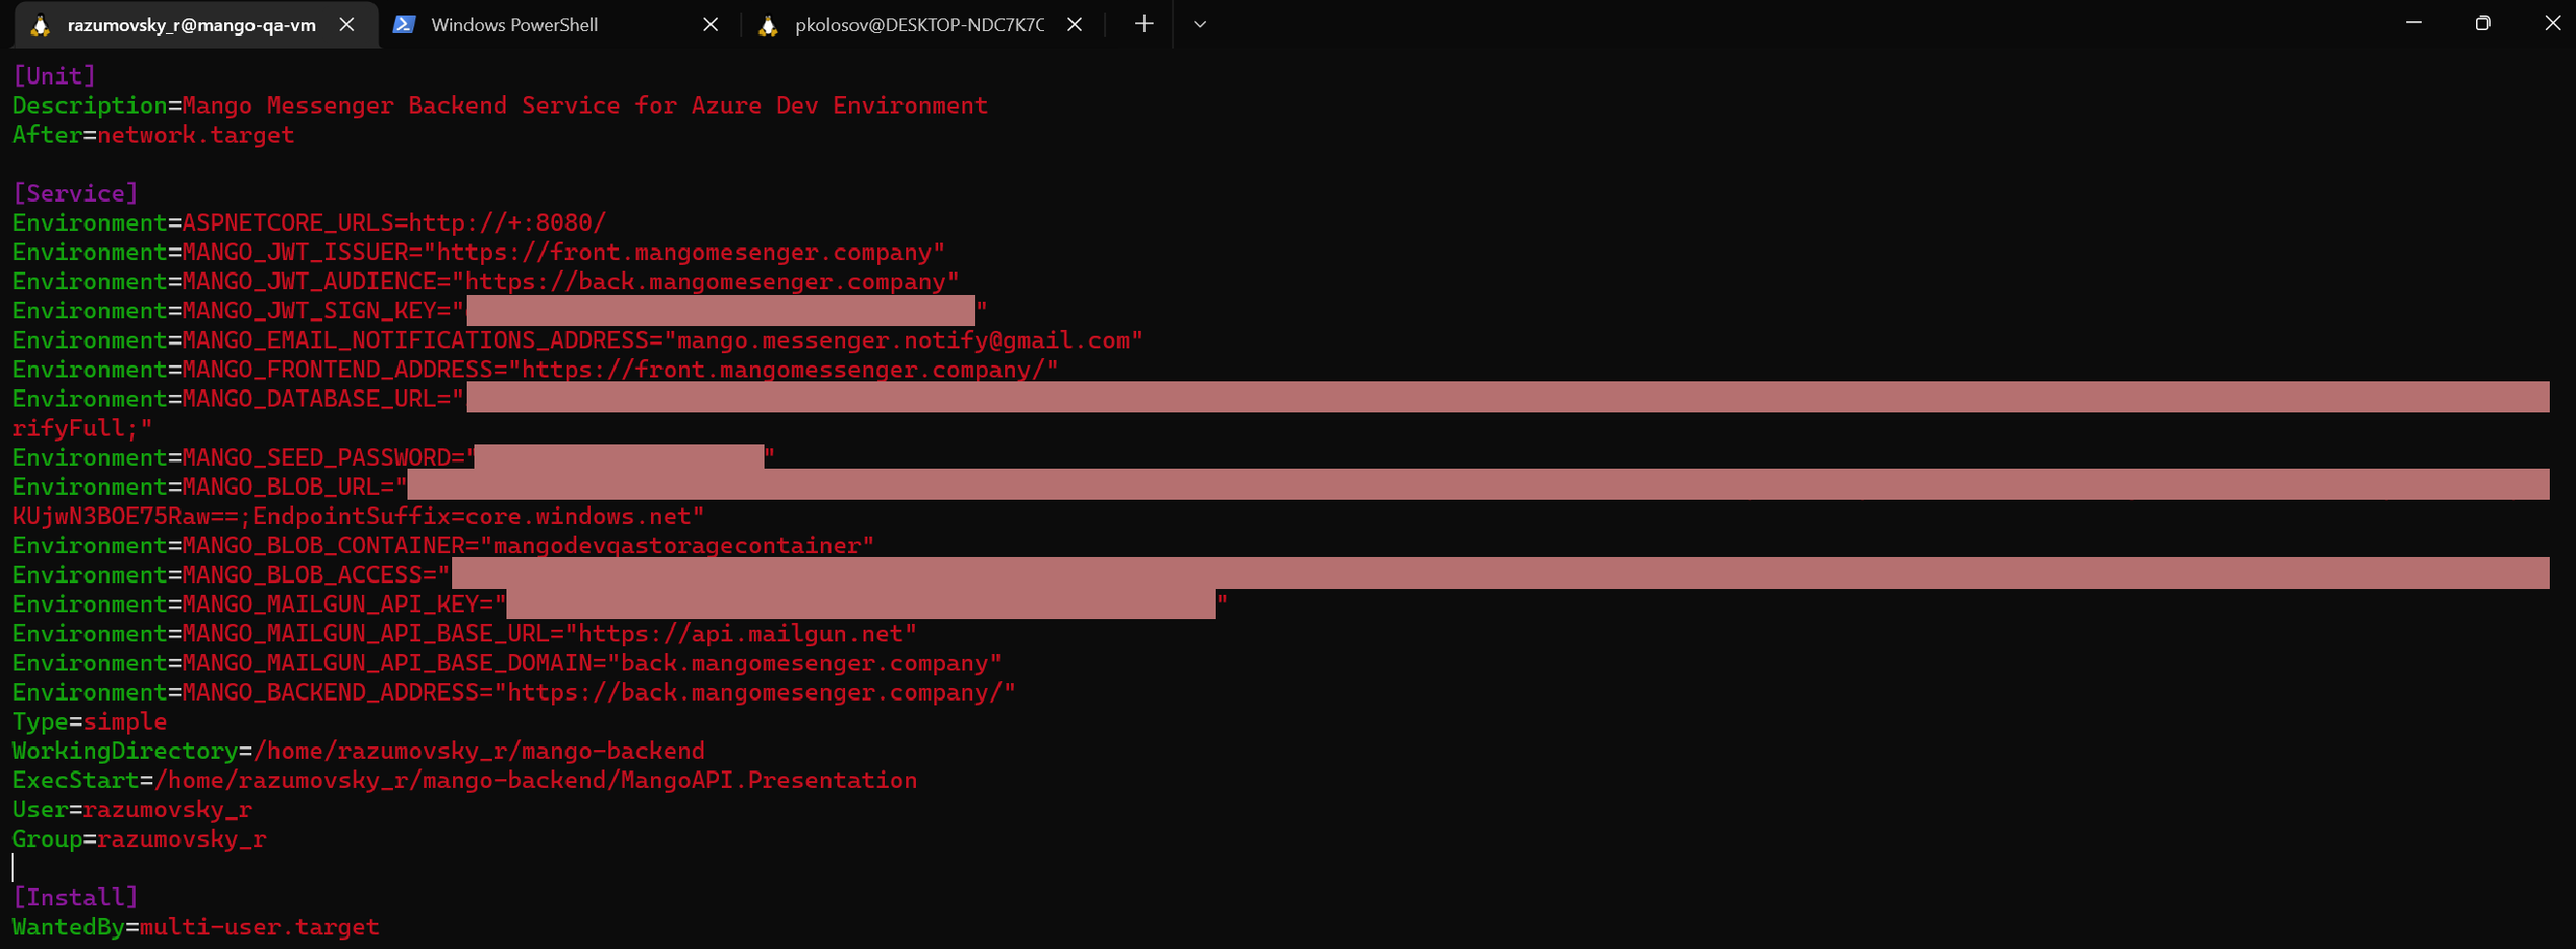
\includegraphics[width=1\textwidth]{img/05_ubuntu_service_vim}
    ~\caption{Ubuntu service opened in vim.}\label{fig:figure13}
\end{figure}
Make sure all resources are listening from the outside, check firewall rules on database side prior to run the service.
Start and check health of the service using
\begin{itemize}
    \item \texttt{sudo systemctl start mangoback}
    \item \texttt{sudo systemctl status mangoback}
\end{itemize}
Terminal output:
\begin{figure}[H]
    \centering
    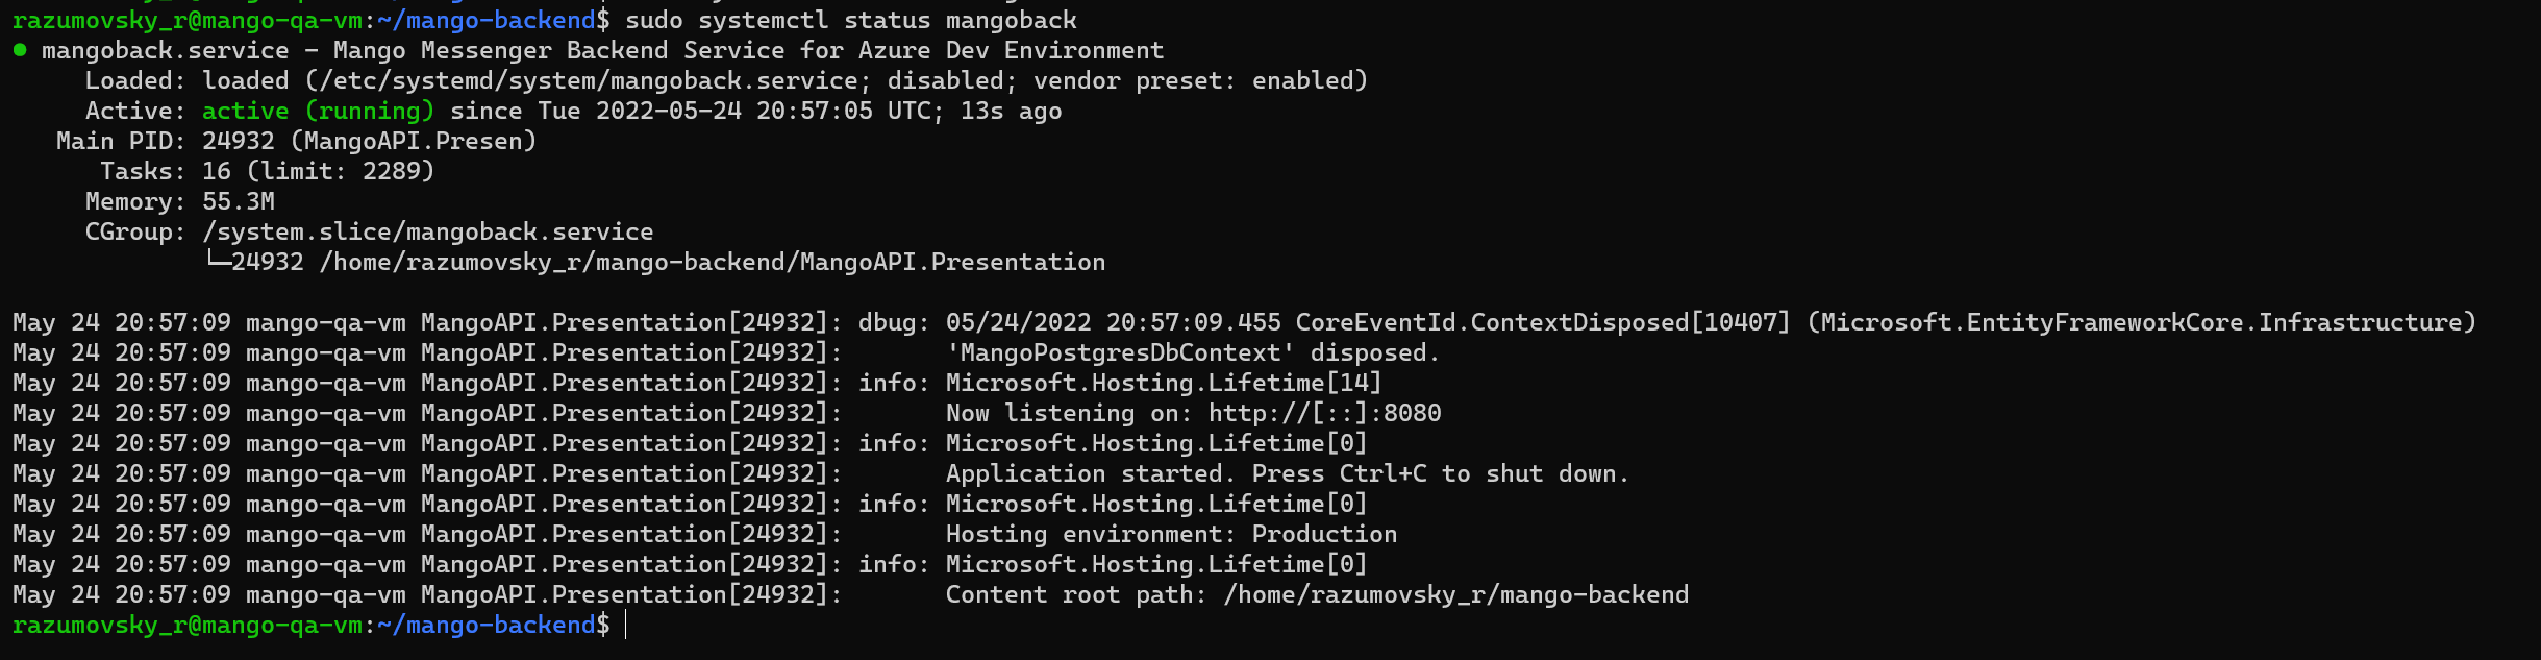
\includegraphics[width=1\textwidth]{img/05_ubuntu_service_status}
    ~\caption{Run ubuntu service and check status, terminal output.}\label{fig:figure14}
\end{figure}
This completes the section.
